\documentclass{article}
\usepackage{listings}
\usepackage{graphicx}
\graphicspath{ {/} }
\begin{document}
\begin{titlepage}
\centering

{\bfseries\LARGE Instituto Polit\'ecnico Nacional \par}
\vspace{1cm}
{\scshape\Large Escuela Superiror de Computaci\'on \par}
\vspace{3cm}
{\scshape\Large Teoria de la Computaci\'on \par}
\vspace{3cm}
{\itshape\Large Pr\'actica 2 \par}
{\itshape\Large Primos \par}
\vfill
{\Large Profesor: \par}
{\Large Genaro Juarez Martinez \par}
{\Large Alumno: \par}
{\Large Alcantara Covarrubias Erik \par}
{\Large Email: erik.alcova@gmail.com \par}
{\Large Grupo: 4SCM6\par}
\vfill
\end{titlepage}

\tableofcontents

\newpage

\section{Introducción}
La base de los automatas, que es el tema central de estudio del primer parcial de la materia, es el poder hablar de lenguajes. Cada ser humano ocupa un lenguaje como el español o el ingles. 
\\Pero los automatas ocupan una definicion diferente para un lenguaje:
\begin{itemize}
    \item Un lenguaje se conforma por un alfabeto.
    \item Un alfabeto es un numero finito de simbolos que tienen un significado.
\end{itemize}

\section{Marco Teorico}

\begin{itemize}
    \item Lenguaje ($\sum$): Conjunto de simbolos que conforman un alfabeto
    \\$\sum = \{ 0, 1\}$ Es un lenguaje conformado por el 0 y el 1.
    \\$\sum = \{A, ..., Z\}$ Es un lenguaje conformado por las letras arabigas.\\
    \item Potencia de un Alfabeto ($\sum^n$): Con esta notacion podemos decir cuantas cadenas de n largo se pueden formulario
    \\$\sum = \{0,1\}$
    \\$\sum^0 = \{\epsilon\}$
    \\$\sum^1 = \{0,1\}$
    \\$\sum^2 = \{00,01,10,11\}$
    \\$\sum^n = \{...\}$\\
    \\Nota: $\sum ^*$ es lo mismo que la union de todas las potencias.
    \\\\$\sum ^*$=$\sum^0\bigcup\sum^1\bigcup\sum^2\bigcup...\bigcup\sum^n$
    \item String: Es una cadena de simbolos finita\\
    \item Cadena vacia $\{\epsilon \}$: Es el string que no contiene ningun elemento\\
    \item Longitud de una string $|abc... \vert $ : Es la cantidad de simbolos que tiene un string\\
    \item Lenguaje(\emph{L}):Es el conjunto de todas las cadenas posibles de nuestro alfabeto.
    \\$\emph{L}\subseteq(\sum)^*$
    \item Permutas ($n!$): Cuando un algoritmo tiene un coste factorial es prácticamente inutilizable para valores no muy
    grandes. Es evidente que $n!$ es extremadamente costoso con respecto a los otros.
    \\$1! = 1$, $2! = 2$, $3! = 6$, $4! = 24$
    
\end{itemize}

\section{Desarrollo}

\subsection{Programa 1 - Universo}
Programar el lenguaje binario definido por los números primos. Dada una ”n” que introduzca el usuario o que
el programa lo determine automáticamente. ”n” determina hasta qué número se desea calcular.
\begin{enumerate}
    \item El programa debe de preguntar si quiere calcular otra ”n” o no y salir hasta que se le especifique.   
    \item La salida debe ser expresada en notación de conjunto, debe ir a un archivo de texto. En un archivo
    especificar el conjunto en binario y en otro el conjunto en decimal.
    \item Del archivo de salida calculado, graficar el número símbolos de cada cadena y otra gráfica de 1s de cada cadena. El eje de las "x" representan el número de cadenas y el eje de las "y" el número de símbolos que tiene cada cadena. 
    \\Al mismo tiempo calcular el logaritmo base 10 de esas dos gráficas, en total serán cuatro gráficas.
\end{enumerate} 

\subsection{Planteamiento}
Dentro del lenguaje de programacion de python se va a realizar este programa porque facilita muchisimo el trabajo con herramientas graficas, el programa es "logicamente" sencillo:
\\Solo es numerar del 0 a n todos los numeros y anotar los que sean primos, sin embargo al realizarlo me di cuenta que si lo sobresimplificaba el tiempo de ejecucion se dispararia mucho.
\\por lo que decidi que hiciera la conversion unicamente si el numero era primo y que en vez de guardarlo todo solo escriba en el archivo los datos que se necesitan y ya.
\subsection{Codigo}

\begin{lstlisting}
import random
import matplotlib.pyplot as plt
import time
import math

#Mausque herramienta para mas tarde: liminf, limmed

def ingerir(unos, largo):
    """Crea las graficas necesarias"""
    
    graficar(unos, "2^n", "# de unos")
    graficar(largo, "2^n", "# de digitos")
    graficar(logrec(unos), "2^n", "log10(# de unos)")
    graficar(logrec(largo), "2^n", "log10(# de digitos)")
    
def logrec(array):
    """Aplica Log base 10 a todos los elementos de un array"""
    aux=[]
    for i in array:
        aux.append(math.log10(int(i)))
    return aux

def graficar(y_axis, titlex, titley):
    """Funcion que crea una grafica"""
    try:
        inicio = time.time()
        ax = plt.subplot()
        plt.xlabel(titlex)
        plt.ylabel(titley)
        plt.title(titlex + " y "+titley)
        ax.plot(y_axis)
        fin = time.time()
        print("El tiempo de ejecucion para la grafica: "+titlex+", "+titley+" es: "+str(fin-inicio))
        plt.savefig("Practica2/"+titlex+titley+".png")
        plt.show()
        
    except (KeyboardInterrupt, BufferError):
        fin = time.time()
        plt.show()
        print("El tiempo de ejecucion para la grafica: "+titlex+", "+titley+" es: "+str(fin-inicio))

def isPrime(n):
    """Funcion para saber si un numero es primo"""
     
    # Corner case
    if (n <= 1):
        return False
 
    # Check from 2 to sqrt(n)
    for i in range(2, int(math.sqrt(n))+1):
        if (n % i == 0):
            return False
 
    return True

def permutaciones(bit):
    """Crea las los numeros binarios y guarda los resultados"""
    
    per_file = open("Practica2/permutaciones.txt", "w")
    per_file.write("L{e\n")
    dec_file = open("Practica2/decimales.txt", "w")
    dec_file.write("L{e\n")
    
    
    inicio = time.time()
    unos = 0
    num_unos = []
    num_digitos = []
    
    while(bit > 1):
        
        try:
            if(isPrime(bit)):
                binary = bin(bit).replace("0b", "")
                per_file.write(","+str(binary)+"\n")
                dec_file.write(","+str(bit)+"\n")
                unos += sum(int(x) for x in binary if x.isdigit())
                
                num_unos.append(unos)  
                num_digitos.append(len(binary))
                del binary
            bit -= 1
            
        except (KeyboardInterrupt,OverflowError):
            break
    
    per_file.write("}")
    per_file.close()
    dec_file.write("}")
    dec_file.close()
    
    fin = time.time()
    
    print("El tiempo de ejecucion es: "+str(fin-inicio))
    ingerir(num_unos, num_digitos[::-1])
        
            
if __name__ == "__main__":
    """Main function"""
    
    while True:
        print("\nMENU")
        print("1) Modo manual")
        print("2) Modo automatico")
        print("3) Salir")
        aux = int(input("Seleccione una opcion: "))
            
        if aux == 1:
            n = int(input("\nIntroduce n, no mayor a 2e7 ni menor a 2: "))
            if 2e7 < n < 2:
                print("Error, el numero introducido no es valido")
                break
            permutaciones(n)
        
        elif aux ==2:
            n = random.randrange(2,2e7)
            permutaciones(n)
            
        elif aux == 3:
            exit()    
        
        else:
            print("Error, seleccione una opcion correcta")
            break

\end{lstlisting}

\section{Resultados}

Los siguientes son los resultados obtenidos al correr el programa con $n = 200^3$:
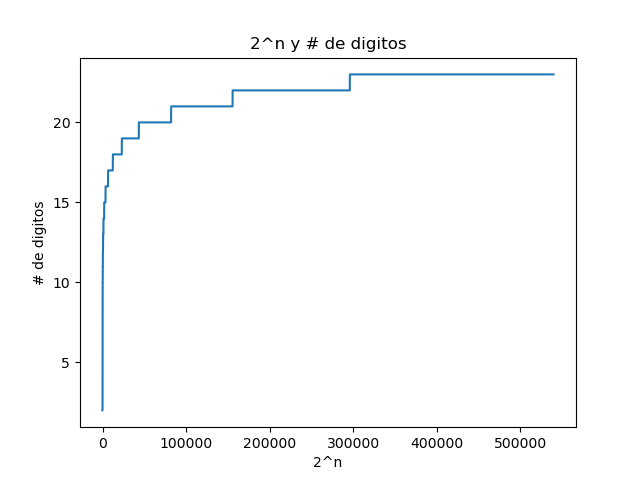
\includegraphics{Graph1.png}
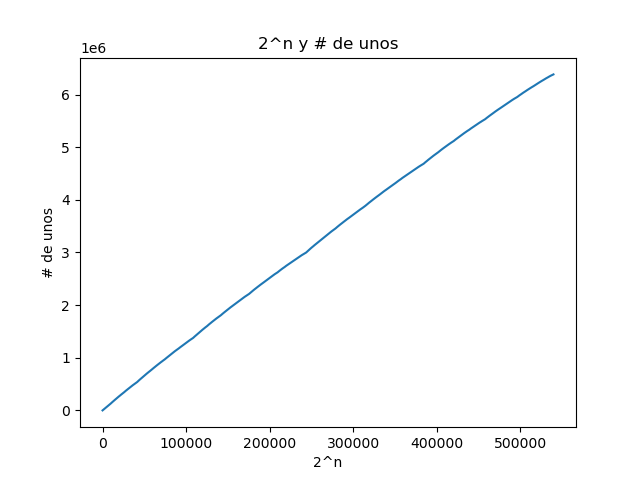
\includegraphics{Graph2.png}
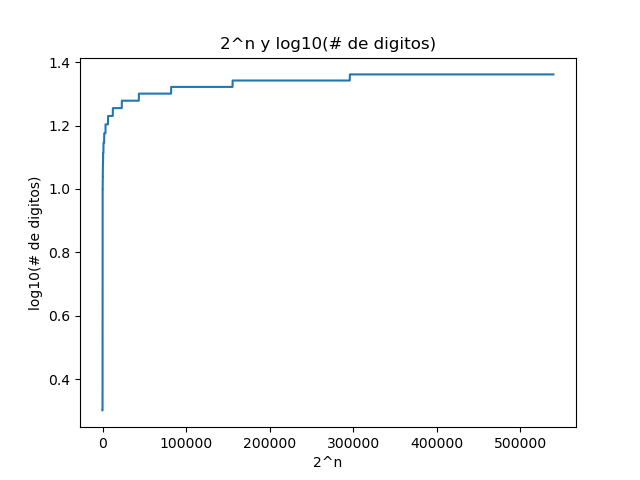
\includegraphics{Graph3.png}
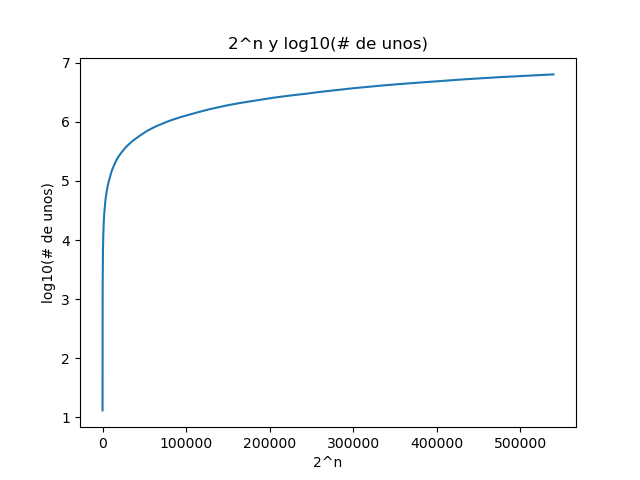
\includegraphics{Graph4.png}
Tambien se crearon 2 archivos .txt que contiene todos los resultados sin embargo pesan $\pm$10gb c/u por lo que no se puede incluir en los extras de este programa.\\
\\Nota: Por motivos de logica el codigo calcula los numeros del mayor al menor, por lo que al realizar las graficas se invirtio el orden de los valores para que no fuera confuso

\section{Conclusión}
El algoritmo no me resulto tan complicado, en primera instancia entendi mal las instrucciones y queria calcular todo el universo de cadenas con $n = 200^3$ por lo que mi algoritmo tarbada casi semanas en acabar.
\\Pero al leer nuevamente que ese era el limite mi programa podia hacer todas las operaciones necesarias en 62s aprox. por lo que muchas de las optimizaciones que ya le habia aplicado hicieron que fuera mucho mas facil terminarlo.
\\Fue entretenido hacer este algoritmo, ademas pude rectificar varios conocimientos previos que fueron necesarios para terminar este proyecto.

\section{Referencias bibliograficas}
\begin{itemize}
    \item LaTeX - A document preparation system. (s. f.). LaTeX - A document preparation system. https://www.latex-project.org/
\end{itemize}
\end{document}